% Generated by Sphinx.
\def\sphinxdocclass{report}
\documentclass[letterpaper,10pt,english]{sphinxmanual}
\usepackage[utf8]{inputenc}
\DeclareUnicodeCharacter{00A0}{\nobreakspace}
\usepackage[T1]{fontenc}
\usepackage{babel}
\usepackage{times}
\usepackage[Bjarne]{fncychap}
\usepackage{longtable}
\usepackage{sphinx}
\usepackage{multirow}


\title{OpenCV-Python Tutorials Documentation}
\date{June 01, 2013}
\release{1}
\author{Alexander Mordvintsev \& Abid K}
\newcommand{\sphinxlogo}{}
\renewcommand{\releasename}{Release}
\makeindex

\makeatletter
\def\PYG@reset{\let\PYG@it=\relax \let\PYG@bf=\relax%
    \let\PYG@ul=\relax \let\PYG@tc=\relax%
    \let\PYG@bc=\relax \let\PYG@ff=\relax}
\def\PYG@tok#1{\csname PYG@tok@#1\endcsname}
\def\PYG@toks#1+{\ifx\relax#1\empty\else%
    \PYG@tok{#1}\expandafter\PYG@toks\fi}
\def\PYG@do#1{\PYG@bc{\PYG@tc{\PYG@ul{%
    \PYG@it{\PYG@bf{\PYG@ff{#1}}}}}}}
\def\PYG#1#2{\PYG@reset\PYG@toks#1+\relax+\PYG@do{#2}}

\expandafter\def\csname PYG@tok@gd\endcsname{\def\PYG@tc##1{\textcolor[rgb]{0.63,0.00,0.00}{##1}}}
\expandafter\def\csname PYG@tok@gu\endcsname{\let\PYG@bf=\textbf\def\PYG@tc##1{\textcolor[rgb]{0.50,0.00,0.50}{##1}}}
\expandafter\def\csname PYG@tok@gt\endcsname{\def\PYG@tc##1{\textcolor[rgb]{0.00,0.27,0.87}{##1}}}
\expandafter\def\csname PYG@tok@gs\endcsname{\let\PYG@bf=\textbf}
\expandafter\def\csname PYG@tok@gr\endcsname{\def\PYG@tc##1{\textcolor[rgb]{1.00,0.00,0.00}{##1}}}
\expandafter\def\csname PYG@tok@cm\endcsname{\let\PYG@it=\textit\def\PYG@tc##1{\textcolor[rgb]{0.25,0.50,0.56}{##1}}}
\expandafter\def\csname PYG@tok@vg\endcsname{\def\PYG@tc##1{\textcolor[rgb]{0.73,0.38,0.84}{##1}}}
\expandafter\def\csname PYG@tok@m\endcsname{\def\PYG@tc##1{\textcolor[rgb]{0.13,0.50,0.31}{##1}}}
\expandafter\def\csname PYG@tok@mh\endcsname{\def\PYG@tc##1{\textcolor[rgb]{0.13,0.50,0.31}{##1}}}
\expandafter\def\csname PYG@tok@cs\endcsname{\def\PYG@tc##1{\textcolor[rgb]{0.25,0.50,0.56}{##1}}\def\PYG@bc##1{\setlength{\fboxsep}{0pt}\colorbox[rgb]{1.00,0.94,0.94}{\strut ##1}}}
\expandafter\def\csname PYG@tok@ge\endcsname{\let\PYG@it=\textit}
\expandafter\def\csname PYG@tok@vc\endcsname{\def\PYG@tc##1{\textcolor[rgb]{0.73,0.38,0.84}{##1}}}
\expandafter\def\csname PYG@tok@il\endcsname{\def\PYG@tc##1{\textcolor[rgb]{0.13,0.50,0.31}{##1}}}
\expandafter\def\csname PYG@tok@go\endcsname{\def\PYG@tc##1{\textcolor[rgb]{0.20,0.20,0.20}{##1}}}
\expandafter\def\csname PYG@tok@cp\endcsname{\def\PYG@tc##1{\textcolor[rgb]{0.00,0.44,0.13}{##1}}}
\expandafter\def\csname PYG@tok@gi\endcsname{\def\PYG@tc##1{\textcolor[rgb]{0.00,0.63,0.00}{##1}}}
\expandafter\def\csname PYG@tok@gh\endcsname{\let\PYG@bf=\textbf\def\PYG@tc##1{\textcolor[rgb]{0.00,0.00,0.50}{##1}}}
\expandafter\def\csname PYG@tok@ni\endcsname{\let\PYG@bf=\textbf\def\PYG@tc##1{\textcolor[rgb]{0.84,0.33,0.22}{##1}}}
\expandafter\def\csname PYG@tok@nl\endcsname{\let\PYG@bf=\textbf\def\PYG@tc##1{\textcolor[rgb]{0.00,0.13,0.44}{##1}}}
\expandafter\def\csname PYG@tok@nn\endcsname{\let\PYG@bf=\textbf\def\PYG@tc##1{\textcolor[rgb]{0.05,0.52,0.71}{##1}}}
\expandafter\def\csname PYG@tok@no\endcsname{\def\PYG@tc##1{\textcolor[rgb]{0.38,0.68,0.84}{##1}}}
\expandafter\def\csname PYG@tok@na\endcsname{\def\PYG@tc##1{\textcolor[rgb]{0.25,0.44,0.63}{##1}}}
\expandafter\def\csname PYG@tok@nb\endcsname{\def\PYG@tc##1{\textcolor[rgb]{0.00,0.44,0.13}{##1}}}
\expandafter\def\csname PYG@tok@nc\endcsname{\let\PYG@bf=\textbf\def\PYG@tc##1{\textcolor[rgb]{0.05,0.52,0.71}{##1}}}
\expandafter\def\csname PYG@tok@nd\endcsname{\let\PYG@bf=\textbf\def\PYG@tc##1{\textcolor[rgb]{0.33,0.33,0.33}{##1}}}
\expandafter\def\csname PYG@tok@ne\endcsname{\def\PYG@tc##1{\textcolor[rgb]{0.00,0.44,0.13}{##1}}}
\expandafter\def\csname PYG@tok@nf\endcsname{\def\PYG@tc##1{\textcolor[rgb]{0.02,0.16,0.49}{##1}}}
\expandafter\def\csname PYG@tok@si\endcsname{\let\PYG@it=\textit\def\PYG@tc##1{\textcolor[rgb]{0.44,0.63,0.82}{##1}}}
\expandafter\def\csname PYG@tok@s2\endcsname{\def\PYG@tc##1{\textcolor[rgb]{0.25,0.44,0.63}{##1}}}
\expandafter\def\csname PYG@tok@vi\endcsname{\def\PYG@tc##1{\textcolor[rgb]{0.73,0.38,0.84}{##1}}}
\expandafter\def\csname PYG@tok@nt\endcsname{\let\PYG@bf=\textbf\def\PYG@tc##1{\textcolor[rgb]{0.02,0.16,0.45}{##1}}}
\expandafter\def\csname PYG@tok@nv\endcsname{\def\PYG@tc##1{\textcolor[rgb]{0.73,0.38,0.84}{##1}}}
\expandafter\def\csname PYG@tok@s1\endcsname{\def\PYG@tc##1{\textcolor[rgb]{0.25,0.44,0.63}{##1}}}
\expandafter\def\csname PYG@tok@gp\endcsname{\let\PYG@bf=\textbf\def\PYG@tc##1{\textcolor[rgb]{0.78,0.36,0.04}{##1}}}
\expandafter\def\csname PYG@tok@sh\endcsname{\def\PYG@tc##1{\textcolor[rgb]{0.25,0.44,0.63}{##1}}}
\expandafter\def\csname PYG@tok@ow\endcsname{\let\PYG@bf=\textbf\def\PYG@tc##1{\textcolor[rgb]{0.00,0.44,0.13}{##1}}}
\expandafter\def\csname PYG@tok@sx\endcsname{\def\PYG@tc##1{\textcolor[rgb]{0.78,0.36,0.04}{##1}}}
\expandafter\def\csname PYG@tok@bp\endcsname{\def\PYG@tc##1{\textcolor[rgb]{0.00,0.44,0.13}{##1}}}
\expandafter\def\csname PYG@tok@c1\endcsname{\let\PYG@it=\textit\def\PYG@tc##1{\textcolor[rgb]{0.25,0.50,0.56}{##1}}}
\expandafter\def\csname PYG@tok@kc\endcsname{\let\PYG@bf=\textbf\def\PYG@tc##1{\textcolor[rgb]{0.00,0.44,0.13}{##1}}}
\expandafter\def\csname PYG@tok@c\endcsname{\let\PYG@it=\textit\def\PYG@tc##1{\textcolor[rgb]{0.25,0.50,0.56}{##1}}}
\expandafter\def\csname PYG@tok@mf\endcsname{\def\PYG@tc##1{\textcolor[rgb]{0.13,0.50,0.31}{##1}}}
\expandafter\def\csname PYG@tok@err\endcsname{\def\PYG@bc##1{\setlength{\fboxsep}{0pt}\fcolorbox[rgb]{1.00,0.00,0.00}{1,1,1}{\strut ##1}}}
\expandafter\def\csname PYG@tok@kd\endcsname{\let\PYG@bf=\textbf\def\PYG@tc##1{\textcolor[rgb]{0.00,0.44,0.13}{##1}}}
\expandafter\def\csname PYG@tok@ss\endcsname{\def\PYG@tc##1{\textcolor[rgb]{0.32,0.47,0.09}{##1}}}
\expandafter\def\csname PYG@tok@sr\endcsname{\def\PYG@tc##1{\textcolor[rgb]{0.14,0.33,0.53}{##1}}}
\expandafter\def\csname PYG@tok@mo\endcsname{\def\PYG@tc##1{\textcolor[rgb]{0.13,0.50,0.31}{##1}}}
\expandafter\def\csname PYG@tok@mi\endcsname{\def\PYG@tc##1{\textcolor[rgb]{0.13,0.50,0.31}{##1}}}
\expandafter\def\csname PYG@tok@kn\endcsname{\let\PYG@bf=\textbf\def\PYG@tc##1{\textcolor[rgb]{0.00,0.44,0.13}{##1}}}
\expandafter\def\csname PYG@tok@o\endcsname{\def\PYG@tc##1{\textcolor[rgb]{0.40,0.40,0.40}{##1}}}
\expandafter\def\csname PYG@tok@kr\endcsname{\let\PYG@bf=\textbf\def\PYG@tc##1{\textcolor[rgb]{0.00,0.44,0.13}{##1}}}
\expandafter\def\csname PYG@tok@s\endcsname{\def\PYG@tc##1{\textcolor[rgb]{0.25,0.44,0.63}{##1}}}
\expandafter\def\csname PYG@tok@kp\endcsname{\def\PYG@tc##1{\textcolor[rgb]{0.00,0.44,0.13}{##1}}}
\expandafter\def\csname PYG@tok@w\endcsname{\def\PYG@tc##1{\textcolor[rgb]{0.73,0.73,0.73}{##1}}}
\expandafter\def\csname PYG@tok@kt\endcsname{\def\PYG@tc##1{\textcolor[rgb]{0.56,0.13,0.00}{##1}}}
\expandafter\def\csname PYG@tok@sc\endcsname{\def\PYG@tc##1{\textcolor[rgb]{0.25,0.44,0.63}{##1}}}
\expandafter\def\csname PYG@tok@sb\endcsname{\def\PYG@tc##1{\textcolor[rgb]{0.25,0.44,0.63}{##1}}}
\expandafter\def\csname PYG@tok@k\endcsname{\let\PYG@bf=\textbf\def\PYG@tc##1{\textcolor[rgb]{0.00,0.44,0.13}{##1}}}
\expandafter\def\csname PYG@tok@se\endcsname{\let\PYG@bf=\textbf\def\PYG@tc##1{\textcolor[rgb]{0.25,0.44,0.63}{##1}}}
\expandafter\def\csname PYG@tok@sd\endcsname{\let\PYG@it=\textit\def\PYG@tc##1{\textcolor[rgb]{0.25,0.44,0.63}{##1}}}

\def\PYGZbs{\char`\\}
\def\PYGZus{\char`\_}
\def\PYGZob{\char`\{}
\def\PYGZcb{\char`\}}
\def\PYGZca{\char`\^}
\def\PYGZam{\char`\&}
\def\PYGZlt{\char`\<}
\def\PYGZgt{\char`\>}
\def\PYGZsh{\char`\#}
\def\PYGZpc{\char`\%}
\def\PYGZdl{\char`\$}
\def\PYGZhy{\char`\-}
\def\PYGZsq{\char`\'}
\def\PYGZdq{\char`\"}
\def\PYGZti{\char`\~}
% for compatibility with earlier versions
\def\PYGZat{@}
\def\PYGZlb{[}
\def\PYGZrb{]}
\makeatother

\begin{document}

\maketitle
\tableofcontents
\phantomsection\label{index::doc}


Contents:


\chapter{OpenCV-Python Tutorials}
\label{py_tutorials/py_tutorials:opencv-python-tutorials}\label{py_tutorials/py_tutorials::doc}\label{py_tutorials/py_tutorials:welcome-to-opencv-python-tutorials-s-documentation}\begin{itemize}
\item {} 
{\hyperref[py_tutorials/py_setup/py_table_of_contents_setup/py_table_of_contents_setup:table-of-content-setup]{\emph{Introduction to OpenCV}}}

\begin{tabulary}{\linewidth}{m{100pt} m{300pt}}
\hline

\includegraphics[width=80pt,height=80pt]{py_tutorials/images/introduction.jpg}
 & 
Learn how to setup OpenCV on your computer!
\\\hline
\end{tabulary}


\item {} 
\emph{Table-Of-Content-Core}

\begin{tabulary}{\linewidth}{m{100pt} m{300pt}}
\hline

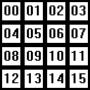
\includegraphics[width=80pt,height=80pt]{py_tutorials/images/core.jpg}
 & 
Here you will learn the about the basic building blocks of the library. A must read and know for     understanding how to manipulate the images on a pixel level.
\\\hline
\end{tabulary}


\item {} 
\emph{Table-Of-Content-ImgProc}

\begin{tabulary}{\linewidth}{m{100pt} m{300pt}}
\hline

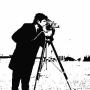
\includegraphics[width=80pt,height=80pt]{py_tutorials/images/imgproc.jpg}
 & 
In this section you will learn about the image processing (manipulation) functions inside OpenCV.
\\\hline
\end{tabulary}


\end{itemize}
\pagebreak

\section{Introduction to OpenCV}
\label{py_tutorials/py_setup/py_table_of_contents_setup/py_table_of_contents_setup:table-of-content-setup}\label{py_tutorials/py_setup/py_table_of_contents_setup/py_table_of_contents_setup:introduction-to-opencv}\label{py_tutorials/py_setup/py_table_of_contents_setup/py_table_of_contents_setup::doc}
Here you can read tutorials about how to set up your computer to work with the OpenCV library.
Additionally you can find a few very basic sample source code that will let introduce you to the
world of the OpenCV.
\begin{itemize}
\item {} 
{\hyperref[py_tutorials/py_setup/py_tutorial_template/py_tutorial_template:tutorial-template]{\emph{Title of Doc comes here}}}

\end{itemize}
\begin{quote}

\begin{tabulary}{\linewidth}{m{100pt} m{300pt}}
\hline

\includegraphics[width=90pt,height=90pt]{py_tutorials/py_setup/py_table_of_contents_setup/images/windows-logo.jpg}
 & 
Template for tutorial doc
\\\hline
\end{tabulary}

\end{quote}
\begin{itemize}
\item {} 
{\hyperref[py_tutorials/py_setup/py_setup_in_windows/py_setup_in_windows:install-opencv-python-in-windows]{\emph{Install OpenCV-Python in Windows}}}

\end{itemize}
\begin{quote}

\begin{tabulary}{\linewidth}{m{100pt} m{300pt}}
\hline

\includegraphics[width=90pt,height=90pt]{py_tutorials/py_setup/py_table_of_contents_setup/images/windows-logo.jpg}
 & 
Set Up OpenCV-Python in Windows
\\\hline
\end{tabulary}

\end{quote}
\begin{itemize}
\item {} 
{\hyperref[py_tutorials/py_setup/py_setup_in_fedora/py_setup_in_fedora:install-opencv-python-in-fedora]{\emph{Install OpenCV-Python in Fedora}}}

\end{itemize}
\begin{quote}

\begin{tabulary}{\linewidth}{m{100pt} m{300pt}}
\hline

\includegraphics[width=90pt,height=90pt]{py_tutorials/py_setup/py_table_of_contents_setup/images/fedora-logo.jpg}
 & 
Set Up OpenCV-Python in Fedora
\\\hline
\end{tabulary}

\end{quote}
\pagebreak

\subsection{Title of Doc comes here}
\label{py_tutorials/py_setup/py_tutorial_template/py_tutorial_template:tutorial-template}\label{py_tutorials/py_setup/py_tutorial_template/py_tutorial_template::doc}\label{py_tutorials/py_setup/py_tutorial_template/py_tutorial_template:title-of-doc-comes-here}

\subsubsection{Goals}
\label{py_tutorials/py_setup/py_tutorial_template/py_tutorial_template:goals}
Explain here following things:
\begin{itemize}
\item {} 
What is this tutorial about ? What you will learn here?

\item {} 
What are all new functions you will see here (eg {\color{red}\bfseries{}:ocv:func:{}`borderInterpolate{}`})

\end{itemize}


\subsubsection{Theory}
\label{py_tutorials/py_setup/py_tutorial_template/py_tutorial_template:theory}\begin{itemize}
\item {} 
Some intuitive explanation of algorithm is given here

\item {} 
If needed, give some equations as inline $g(i,j)$ or next line as,

\end{itemize}
\begin{gather}
\begin{split}g(i,h) = \sum_{k,l} f(i+k, j+l) h(k,l)\end{split}\notag\\\begin{split}\end{split}\notag
\end{gather}\begin{itemize}
\item {} 
If required, a Numpy implementation of algorithm also can be given as a separate subsection

\end{itemize}


\paragraph{Subsection Python Implementation {[}optional{]}}
\label{py_tutorials/py_setup/py_tutorial_template/py_tutorial_template:subsection-python-implementation-optional}
Numpy code comes here. To add code, do as follows :

\begin{Verbatim}[commandchars=\\\{\}]
\PYG{k+kn}{import} \PYG{n+nn}{cv2}
\PYG{k+kn}{import} \PYG{n+nn}{numpy} \PYG{k+kn}{as} \PYG{n+nn}{np}

\PYG{k}{print} \PYG{l+s}{\PYGZsq{}}\PYG{l+s}{import done}\PYG{l+s}{\PYGZsq{}}
\end{Verbatim}


\subsubsection{OpenCV sample}
\label{py_tutorials/py_setup/py_tutorial_template/py_tutorial_template:opencv-sample}
Here comes the original OpenCV code with explanation. Result also can included in this itself.

To add image, do as follows :
\begin{quote}

{\hfill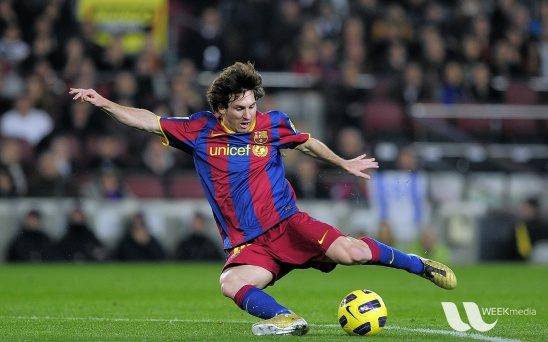
\includegraphics{messi5.jpg}\hfill}
\end{quote}

Notes, warnings, Todo etc can be done as follows :

\begin{notice}{note}{Note:}
The explanation below belongs to the book
\end{notice}

\begin{notice}{warning}{Warning:}
The explanation below belongs to the book
\end{notice}

\begin{notice}{note}{Todo}

The explanation below belongs to the book
\end{notice}


\strong{See Also:}


The explanation below belongs to the book



external urls are given as \href{http://www.python.org}{Python} which points to python site.

Internal url is called as {\hyperref[py_tutorials/py_setup/py_tutorial_template/py_tutorial_template:tutorial-template]{Tutorial-Template}}

A book is cited as {\hyperref[py_tutorials/py_setup/py_tutorial_template/py_tutorial_template:szeliski]{{[}Szeliski{]}}}


\subsubsection{Common Errors {[}optional{]}}
\label{py_tutorials/py_setup/py_tutorial_template/py_tutorial_template:common-errors-optional}
We can show solutions for some common mistakes while using certain functionalities, if any.


\subsubsection{Exercises {[}optional{]}}
\label{py_tutorials/py_setup/py_tutorial_template/py_tutorial_template:exercises-optional}
Here we can give some additional tasks for reader to do
\begin{itemize}
\item {} 
like read and understand more advanced code on the same algorithm.

\item {} 
Related SOF and answers.opencv.org questions

\item {} 
Our own questions or tasks

\end{itemize}


\subsubsection{References {[}optional{]}}
\label{py_tutorials/py_setup/py_tutorial_template/py_tutorial_template:references-optional}
Give references if any for better understanding of algorithm, like any standard textbooks, web links etc. Numbered references are given as
\begin{enumerate}
\item {} 
Learning OpenCV

\item {} 
Computer Vision Models

\end{enumerate}


\subsection{Install OpenCV-Python in Windows}
\label{py_tutorials/py_setup/py_setup_in_windows/py_setup_in_windows:install-opencv-python-in-windows}\label{py_tutorials/py_setup/py_setup_in_windows/py_setup_in_windows::doc}\label{py_tutorials/py_setup/py_setup_in_windows/py_setup_in_windows:id1}

\subsubsection{Goals}
\label{py_tutorials/py_setup/py_setup_in_windows/py_setup_in_windows:goals}
In this tutorial, you will learn to setup OpenCV-Python in your Windows system. Below steps are tested for Windows 7.


\subsubsection{Required Packages}
\label{py_tutorials/py_setup/py_setup_in_windows/py_setup_in_windows:required-packages}\begin{enumerate}
\item {} 
Python

\item {} 
Numpy

\item {} 
OpenCV

\end{enumerate}

Below are some optional packages which will be useful in your journey.
\begin{enumerate}
\item {} 
Matplotlib

\item {} 
SciPy

\end{enumerate}

Install Python, Numpy, Matplotlib, Scipy to their default locations. To install OpenCV, you can either use prebuilt binaries or compile from source.


\subsubsection{Installing OpenCV from prebuilt binaries}
\label{py_tutorials/py_setup/py_setup_in_windows/py_setup_in_windows:installing-opencv-from-prebuilt-binaries}\begin{enumerate}
\item {} 
Goto opencv/../../2.7 folder.

\item {} 
Copy cv2.pyd to C:/Python27/lib/site-packeges

\item {} 
Open Python IDLE and type following codes in Python terminal.

\begin{Verbatim}[commandchars=\\\{\}]
\PYG{g+gp}{\PYGZgt{}\PYGZgt{}\PYGZgt{} }\PYG{k+kn}{import} \PYG{n+nn}{cv2}
\PYG{g+gp}{\PYGZgt{}\PYGZgt{}\PYGZgt{} }\PYG{k}{print} \PYG{n}{cv2}\PYG{o}{.}\PYG{n}{\PYGZus{}\PYGZus{}version\PYGZus{}\PYGZus{}}
\end{Verbatim}

\end{enumerate}

If the results are printed out without any errors, congratulations !!! You have installed OpenCV-Python successfully.


\subsubsection{Installing OpenCV from source}
\label{py_tutorials/py_setup/py_setup_in_windows/py_setup_in_windows:installing-opencv-from-source}\begin{enumerate}
\item {} 
Put complete compilation steps here

\end{enumerate}


\subsection{Install OpenCV-Python in Fedora}
\label{py_tutorials/py_setup/py_setup_in_fedora/py_setup_in_fedora::doc}\label{py_tutorials/py_setup/py_setup_in_fedora/py_setup_in_fedora:install-opencv-python-in-fedora}\label{py_tutorials/py_setup/py_setup_in_fedora/py_setup_in_fedora:id1}

\subsubsection{Goals}
\label{py_tutorials/py_setup/py_setup_in_fedora/py_setup_in_fedora:goals}
In this tutorial, you will learn to setup OpenCV-Python in your Fedora system. Below steps are tested for Fedora 18.


\subsubsection{Required Packages}
\label{py_tutorials/py_setup/py_setup_in_fedora/py_setup_in_fedora:required-packages}\begin{enumerate}
\item {} 
Python

\item {} 
Numpy

\item {} 
OpenCV

\end{enumerate}

Below are some optional packages which will be useful in your journey.
\begin{enumerate}
\item {} 
Matplotlib

\item {} 
SciPy

\end{enumerate}

Install Python, Numpy, Matplotlib, Scipy to their default locations. To install OpenCV, you can either use prebuilt binaries or compile from source.


\subsubsection{Installing OpenCV from prebuilt binaries}
\label{py_tutorials/py_setup/py_setup_in_fedora/py_setup_in_fedora:installing-opencv-from-prebuilt-binaries}\begin{enumerate}
\item {} 
Install all packages with following command in terminal as root.

\end{enumerate}

\begin{Verbatim}[commandchars=\\\{\}]
yum install python\PYGZhy{}numpy opencv opencv\PYGZhy{}python
\end{Verbatim}
\begin{enumerate}
\item {} 
Open Python IDLE and type following codes in Python terminal.

\begin{Verbatim}[commandchars=\\\{\}]
\PYG{g+gp}{\PYGZgt{}\PYGZgt{}\PYGZgt{} }\PYG{k+kn}{import} \PYG{n+nn}{cv2}
\PYG{g+gp}{\PYGZgt{}\PYGZgt{}\PYGZgt{} }\PYG{k}{print} \PYG{n}{cv2}\PYG{o}{.}\PYG{n}{\PYGZus{}\PYGZus{}version\PYGZus{}\PYGZus{}}
\end{Verbatim}

\end{enumerate}

If the results are printed out without any errors, congratulations !!! You have installed OpenCV-Python successfully.


\subsubsection{Installing OpenCV from source}
\label{py_tutorials/py_setup/py_setup_in_fedora/py_setup_in_fedora:installing-opencv-from-source}\begin{enumerate}
\item {} 
Put complete compilation steps here

\end{enumerate}


\chapter{Indices and tables}
\label{index:indices-and-tables}\label{index::doc}\begin{itemize}
\item {} 
\emph{genindex}

\item {} 
\emph{modindex}

\item {} 
\emph{search}

\end{itemize}

\begin{thebibliography}{Szeliski}
\bibitem[Szeliski]{Szeliski}{\phantomsection\label{py_tutorials/py_setup/py_tutorial_template/py_tutorial_template:szeliski} 
Computer Vision Models
}
\end{thebibliography}



\renewcommand{\indexname}{Index}
\printindex
\end{document}
